
\documentclass[]{report}
\voffset=-1.5cm
\oddsidemargin=0.0cm
\textwidth = 480pt


\usepackage{amsmath}
\usepackage{graphicx}
\usepackage{amssymb}
\usepackage{framed}
\usepackage{multicol}
%\usepackage[paperwidth=21cm, paperheight=29.8cm]{geometry}
%\usepackage[angle=0,scale=1,color=black,hshift=-0.4cm,vshift=15cm]{background}
%\usepackage{multirow}
\usepackage{enumerate}

\usepackage{amsmath,amsfonts,amssymb}
\usepackage{color}
\usepackage{multirow}
\usepackage{eurosym}
\usepackage{framed}

%\input def.tex
%\input dsdef.tex
%\input rgb.tex

%\newcommand \la{\lambda}
%\newcommand \al{a}
%\newcommand \be{b}
\newcommand \x{\overline{x}}
\newcommand \y{\overline{y}}

\begin{document}
	
%%- http://www3.ul.ie/ramsey/Lectures/Operations_Research_2/gametheory1.pdf

\chapter{CHAPTER - GAME THEORY}
\section{The Concept of a Game}
%%- David Ramsey Section 3.1
Game Theory (GT) is the study of strategic interdependence. 
\begin{framed}
\noindent A game is defined by
\begin{itemize}
	\item[(a)] The set of players (at least two ``\textbf{\textit{rational}}" players).
	\item[(b)] The set of actions available to each player (each has at least
	two possible actions).
	\item[(c)] A payoff function, which gives the (expected) payoff of each
	player given the actions used by the players. The (expected) payoff
	of a player does depend on the actions used by the other players.
\end{itemize}
\end{framed}
\noindent The typical ``game'' consists of players, actions, strategies and payoffs. The standard modes of analysis are once-played games in either
\begin{enumerate}
	\item[(i)] matrix or strategic form where players' choice of actions are made simultaneously,
	\item[] \hspace*{50mm} or
	\item[(ii)] extensive form where choice of actions are made sequentially.
\end{enumerate}


%%- 1 / 45
%-----------------------------------------------------------%
%% \section{3.1 The Concept of a Game}
\begin{itemize}
	\item According to such a definition, roulette is not a mathematical
	game, since the expected winnings of a player only depend on how
	they play.
	\item The lottery is a mathematical game. Although the probability of
	winning the jackpot is independent of the choices of other players,
	a player can maximise his/her expected reward by choosing
	combinations of numbers that other individuals do not choose
	(such an individual is not more likely to win the jackpot, but when
	they win, they win more on average).
\end{itemize}


%===============================================%
%- http://www.investopedia.com/articles/financial-theory/08/game-theory-basics.asp

Game theory is the process of modeling the strategic interaction between two or more players in a situation containing set rules and outcomes. While used in a number of disciplines, game theory is most notably used as a tool within the study of economics. The economic application of game theory can be a valuable tool to aide in the fundamental analysis of industries, sectors and any strategic interaction between two or more firms. Here, we'll take an introductory look at game theory and the terms involved, and introduce you to a simple method of solving games, called backwards induction.

\subsection{Definitions} 
Any time we have a situation with two or more players that involves known payouts or quantifiable consequences, we can use game theory to help determine the most likely outcomes. 
Let's start out by defining a few terms commonly used in the study of game theory:

\begin{description}
	\item[Game:] Any set of circumstances that has a result dependent on the actions of two of more decision makers ("players")
	\item[Players:] A strategic decision maker within the context of the game
	\item[Strategy:] A complete plan of action a player will take given the set of circumstances that might arise within the game
	\item[Payoff:] The payout a player receives from arriving at a particular outcome. The payout can be in any quantifiable form, from dollars to utility.
	\item[Information Set:] The information available at a given point in the game. The term information set is most usually applied when the game has a sequential component.
	\item[Equilibrium:] The point in a game where both players have made their decisions and an outcome is reached.
\end{description}

\subsection{Assumptions}
As with any concept in economics, there is the assumption of rationality. There is also an assumption of maximization. It is assumed that players within the game are rational and will strive to maximize their payoffs in the game. (The question of rationality has been applied to investor behavior as well. Read Understanding Investor Behavior to learn more.)

When examining games that are already set up, it is assumed on your behalf that the payouts listed include the sum of all payoffs that are associated with that outcome. This will exclude any "what if" questions that may arise.

The number of players in a game can theoretically be infinite, but most games will be put into the context of two players. One of the simplest games is a sequential game involving two players.

%-----------------------------------------------------------%
%% 2 / 45
%===========================================================%
\section{3.2 The Matrix Form of a 2-Player Game}
\begin{itemize}
	\item Assume that each player has a finite set of actions to choose from.
	\item In the matrix form of a 2-player game, each row corresponds to an
	action of Player 1 and each column corresponds to an action of
	Player 2.
	\item Each cell of the payoff matrix is associated with a payoff vector.
	The i-th component of this vector gives the payoff to Player i.
\end{itemize}


%% 3 / 45

%===========================================================%
%% 3.2 The Matrix Form of a 2-Player Game
For example, the following describes a so called \textbf{\textit{Hawk-Dove}} game


	\begin{center}
		{\color{blue}
			\begin{tabular}{c|c|c|c|}
				\multicolumn{2} {c} {} & \multicolumn{2}{c} {{\color{red}Player 2}} \\
				\cline{3-4}
				\multicolumn{2}{c|}{} & Hawk         & Dove      \\
				\cline{2-4}
				\multirow{2} {*} {{\color{red}Player 1}}& Hawk & (-2,-2)&  (4,0) \\
				\cline{2-4}
				& Dove &(0,4)& (2,2)\\
				\cline{2-4}
				%C & (2,6) & (4,7)& (0,8) \\
				%\hline
			\end{tabular}
		}
	\end{center}
	
For example, when Player 1 plays H and Player 2 plays D, Player 1
obtains a payoff of 4 and Player 2 obtains a payoff of 0.

%-----------------------------------------------------------%
%% 4 / 45
%%- \section{3.2 The Matrix Form of a 2-Player Game}
In general, a 2-player matrix game can be described by
\begin{enumerate}
	\item The set of actions available to Player 1,
	\[A = \{a_1, a_2, \ldots , a_m\}\].
\item The set of actions available to Player 2,
	\[B = \{b_1, b_2, \ldots , b_n\}\].
\item The m × n matrix of 2-dimensional vectors giving the
	payoffs of both players for each of the m × n possible
	combinations of actions. 
\item The payoff of Player k when
	Player 1 plays ai and Player 2 plays bj will be
	denoted Rk (ai
	, bj).
	
\end{enumerate}

%-----------------------------------------------------------%
%% 5 / 45
%% 3.2 The Matrix Form of a 2-Player Game
\begin{itemize}
	\item One advantage of the matrix form of a game is its simplicity.
	\item One disadvantage is that it is assumed that players choose their
	actions simultaneously.
	\item That is to say, the actions may be
	interpreted as strategies which are chosen at the beginning of a
	game.
	\item As we continue through this chapter, we will differentiate between
	the concept of action and the concept of strategy.
	
\end{itemize}

%-----------------------------------------------------------%
% 6 / 45
\section{Zero-sum and Constant-sum Games}
\begin{itemize}
	\item A game is said to be a constant sum game, if the sum of the
	payoffs obtained by the players is fixed, regardless of the
	combination of strategies used.
	\item	A game is said to be a zero-sum game, if the sum of payoffs
	obtained by the players is always 0, regardless of the combination
	of strategies used.
	\item A game of constant sum k is essentially the same as a zero-sum
	game. A referee could pay both of the players k/2 and require that
	they play the game in which each payoff is reduced by k/2 (this
	would be a zero-sum game).
	\item	2-player constant-sum games are games of pure conflict.
	Whatever one player gains, the other will lose.
\end{itemize}

%% 7 / 45
%%- David Ramsey Section 3.3 
%==========================================================%
\section{The Extensive Form of a Game}
\begin{itemize}
	\item In many games, e.g. chess, each player makes a sequence of moves.
	Such a game can be represented by a tree. 
		\item  Each node represents a
	position (state) in which a player must make a move.
	\item 	Each edge coming out of a node represents a move that the player
	can make in that particular state.
	\item 	Each terminal point of the tree is associated with a payoff vector.
\end{itemize}

%% 8 / 45
%==========================================================%

%%\subsection{The Asymmetric Hawk-Dove Game}


\begin{figure}[h!]
\centering
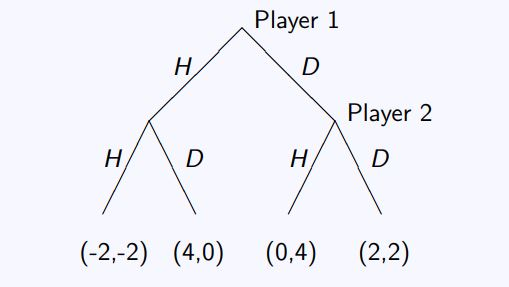
\includegraphics[width=0.55\linewidth]{images/DR5-Slide09}
\caption{}
\label{fig:DR5-Slide09}
\end{figure}


%% 9 / 45
%% The Asymmetric Hawk-Dove Game
\begin{itemize}
	\item In such a game, Player 1 first decides whether to play H and D.
	\item After observing the decision of Player 1, Player 2 then decides
	whether to play H and D.
	\item For example, if Player 1 chooses H and Player 2 chooses D, Player
	1 obtains a payoff of 4 and Player 2 obtains a payoff of 0.
\end{itemize}


\subsection{The Asymmetric Hawk-Dove Game}
%-----------------------------------------------------------%
%% 10 / 45

\begin{itemize}
\item It might appear that this game is equivalent to the matrix form of
	the Hawk-Dove given above.
\item In order to see the difference between these games, we should
	differentiate between strategies and actions.
\item In a game represented in extensive form, a strategy is a rule that
	defines which action a player should play at all the nodes where
	he/she makes a move.
\item An action is the observed behaviour resulting from such a strategy.
\end{itemize}


%-----------------------------------------------------------%
%% 11 / 45
\begin{itemize}
	\item Here Player 1 first chooses between H and D. This is her only
	choice. 
	\item Thus Player 1’s strategies correspond exactly to her
	possible actions (H and D).
	However, since Player 2 observes the move made by Player 1, he
	can condition his move on the move made by Player 1.
	\item For each of the moves made by Player 1, Player 2 has 2 possible
	moves. Hence, he has $2 \times 2 = 4$ possible strategies. These are
	listed on the following slide.
\end{itemize}


%-----------------------------------------------------------%
% 12 / 45
In the extended game described above, Player 2’s strategies are
\begin{enumerate}
	\item  $H|H$, $H|D$, i.e. play H when Player 1 plays H and
	play H when Player 1 plays D, in other words always
	play H.
	\item  $H|H$, $D|D$, i.e. take the same action as Player 1.
	\item  D|H, $D|D$, i.e. always play D.
	\item  D|H, $H|D$, i.e. play D when Player 1 plays H and
	play H when Player 1 plays D.
\end{enumerate}

In the matrix game presented earlier, Player 2 cannot condition his
action on the action made by Player 1. Hence, he only has 2
strategies corresponding to the two actions H and D.

%-----------------------------------------------------------%
%% 13 / 45
\subsection{Simultaneous Moves in Extensive Form Games}
\begin{itemize}
	\item Although the extensive form of the game is designed to describe
	games in which a sequence of moves are made, they can be
	adapted to describe games in which moves are made
	simultaneously.
	\item This is done using information sets. Suppose two nodes represent
	states in which one player moves and that player cannot
	differentiate between the states.
	\item These two nodes are said to be in the same information set. An
	information set is represented by a box.
	\item A player may only condition an action on the information set,
	he/she is presently in.
\end{itemize}


%-----------------------------------------------------------%
%% - 14 / 45


\begin{figure}[h!]
\centering
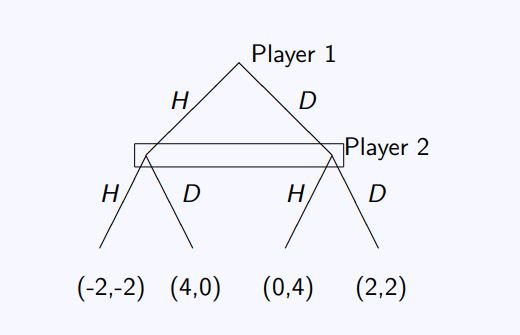
\includegraphics[width=0.55\linewidth]{images/DR5-Slide15}
\caption{}
\label{fig:DR5-Slide15}
\end{figure}
In this case both players have 2 possible strategies: H and D.

%-----------------------------------------------------------%
%% 15 / 45
\subsection{Translating from Extensive Form into Matrix Form}
In order to translate the description of a game from extensive form
to matrix form, we
\begin{enumerate}
\item  List the possible strategies of both players.
\item In the matrix describing the game, the rows
correspond to the strategies of Player 1 and the
columns correspond to the strategies of Player 2.
\item We then derive the payoff vector corresponding to
each possible strategy pair.
\end{enumerate}
%-----------------------------------------------------------%
%% 16 / 45
\begin{itemize}
	\item It should be noted that each game in extensive form has a unique
	definition as a matrix game (apart from possible differences in the
	labelling of the strategies).
\item However, there may be various games in extensive form
	corresponding to a game given in matrix form. 
\item Thus it is generally
	not possible to translate a game in matrix form into a game in
	extensive form.
\item This is unsurprising, since the extensive form of a game gives more
	detailed description of how the game is actually played.
\end{itemize}


%-----------------------------------------------------------%
%% 17 / 45
%%- \subsection{Translating the Asymmetric Hawk-Dove Game into Matrix Form}
\begin{itemize}
	\item Since Player 1 has 2 strategies and Player 2 has 4 strategies, the
	payoff matrix will be of dimension $2 \times 4$.
	\item Player 1 can play H or D.
	\item 	Player 2 can play \[(H|H, H|D), (H|H, D|D), (D|H, D|D) or
	(D|H, H|D). \]
\end{itemize}

%-----------------------------------------------------------%
%% 18 / 45
%% \subsection{Translating the Asymmetric Hawk-Dove Game into Matrix Form}
We now consider the payoff vectors associated with each strategy
pair.
\begin{framed}
\noindent Suppose Player 1 plays H.
\begin{itemize}
	\item[(a)] If Player 2 plays $(H|H, H|D)$ or $(H|H, D|D)$, then both players
take the action H and the resulting payoff vector is (−2, −2).
	\item[(b)] If Player 2 plays (D|H, D|D) or $(D|H, H|D)$, then Player 1
takes the action H and Player 2 takes the action D and the
resulting payoff vector is (4, 0).
\end{itemize}
\end{framed}

%-----------------------------------------------------------%
%19 / 45
%Translating the Asymmetric Hawk-Dove Game into Matrix Form
Now suppose Player 1 plays D.
\begin{itemize}
	\item[(a)] If Player 2 plays $(D|H, D|D)$ or $(H|H, D|D)$, then both players
	take the actions D and the resulting payoff vector is (2, 2).
	\item[(b)] If Player 2 plays $(H|H, H|D)$ or $(D|H, H|D)$, then Player 1 takes
	the action D and Player 2 takes the action H and the resulting
	payoff vector is (0, 4).
\end{itemize}

%-----------------------------------------------------------%
% 20 / 45
%% Translating the Asymmetric Hawk-Dove Game into Matrix Form
It follows that the matrix form of the asymmetric game is given by
\[(H|H, H|D) (H|H, D|D) (D|H, D|D) (D|H, H|D)\]
H (-2,-2) (-2,-2) (4,0) (4,0)
D (0,4) (2,2) (2,2) (0,4)

%-----------------------------------------------------------%
%% 21 / 45
\subsection{Moves by ”Nature”}
\begin{itemize}
	\item Extensive form can also be used to describe moves by ”nature”,
	i.e. random events, the roll of a die, dealing cards.
\item Whenever nature is called to make a move at a given node, the
	edges from this node correspond to the possible results. The
	probability of each result should also be given.
\item When such a game is written in matrix form, we only consider the
	strategies that the players can use. 
\item In order to define the vector of
	expected payoffs given the combination of strategies used, we
	take expectations with respect to the moves of nature (i.e. nature
	is assumed to be ”\textbf{random}” or ”\textbf{non-rationa}l”).
\end{itemize}



%-----------------------------------------------------------%
%% 22 / 45
\subsection{Example}
\begin{itemize}
	\item Suppose that player 1 can first choose either A or B. Player 2 does
	not know this choice.
\item Afterwards Player 2 observes the result of a coin toss. Regardless
	of the result of the coin toss, Player 2 can play A or B.
\item If the coin toss results in heads, when both players choose the
	same action Player 1 obtains \$1 from Player 2, but gives Player 2
	\$1 if each chooses different actions. 
\item If the coin toss results in tails,
	when each player chooses different actions Player 1 obtains \$2
	from Player 2, otherwise he gives Player 2 \$2 (note this is a
	zero-sum game).
\end{itemize}


%-----------------------------------------------------------%23 / 45
%%- \subsection{Example}
\begin{itemize}
	\item When writing the game in extensive form, we can often shift a
	move to an different position in the tree than its natural position,
	in order to make a more legible tree.
	\item	The important thing here is to correctly describe what information
	each player has when making a move.
	\item In this example, Player 1 does not know the result of the coin toss
	(or Player 2’s move).
	\item	Player 2 does not know Player 1’s move, but knows the result of
	the coin toss. 
	\item Hence, Player 2’s move must come lower down the
	tree than the coin toss. We can order the moves as follows:
	nature, Player 1, Player 2.
\end{itemize}

%% 24 / 45
%% Example

\begin{figure}
\centering
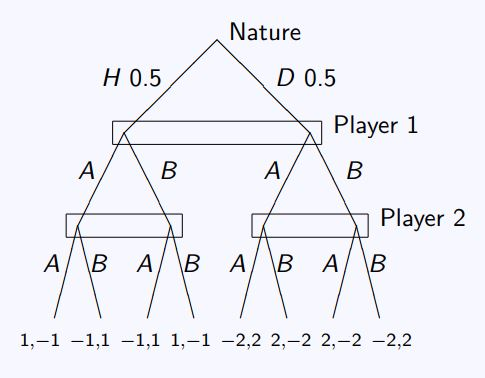
\includegraphics[width=0.55\linewidth]{images/DR5-Slide25}
\caption{}
\label{fig:DR5-Slide25}
\end{figure}

%====================================================%
%% 25 / 45
%% Example
\begin{itemize}
	\item In order to describe the game in matrix form, note that Player 1
	has no information regarding the coin toss or Player 2’s move. It
	follows that she has 2 strategies: A and B.
\item	Player 2 has no information regarding Player 1’s move, but knows
	the result of the coin toss. 
\item Hence, his action can be made
	conditional on the result of the coin toss. He has 4 strategies:
\end{itemize}

\[(A|H, A|T), (A|H, B|T), (B|H, B|T), (B|H, A|T).\]

%-----------------------------------------------------------%
%%26 / 45
%%Example
\begin{itemize}
	\item Suppose Player 1 plays A.
	\item	When Player 2 plays (A|H, A|T), i.e. always A, Player 1 wins 1 if
	the result of the coin toss was H and loses 2 if the result of the
	coin toss was tails. Player 1’s expected reward is
	$0.5 × 1 − 0.5 × 2 = −0.5$. 
	\item Since the game is zero-sum, Player 2’s
	expected payoff is 0.5.
	\item	When Player 2 plays (B|H, B|T), i.e. always B, Player 1 loses 1 if
	the result of the coin toss was H and wins 2 if the result of the
	coin toss was tails. Player 1’s expected reward is
	$0.5 × 2 − 0.5 × 1 = 0.5$.
	\item	The expected rewards under all the other possible pairs of
	strategies can be calculated in a similar way.
\end{itemize}
%%- 27 / 45
%-----------------------------------------------------------%


\subsection{Example}
The matrix form of this game is given by
(A|H, A|T) (A|H, B|T) (B|H, B|T) (B|H, A|T)
A (-0.5,0.5) (1.5,-1.5) (0.5,-0.5) (-1.5,1.5)
B (0.5,-0.5) (-1.5,1.5) (-0.5,0.5) (1.5,-1.5)

%% 28 / 45
%-----------------------------------------------------------%
\subsection{Extensive Forms of Games with a Continuum of Strategies}
Consider the following game:
\begin{itemize}
	\item Player 1 chooses a number x between 0 and 1. Having observed
	the choice of Player 1, Player 2 chooses a number y between 0 and
	1.
	\item The payoff of Player 1 is given by $R1(x, y) = 4xy − x$. 
	\item The payoff
	of Player 2 is given by $R2(x, y) = 4xy − y$.
	\item In order to depict choice from a continuum, instead of using
	branches we can use a triangle with a horizontal base. The
	strategy set is described alongside the corresponding triangle.
\end{itemize}
%% 29 / 45
%-----------------------------------------------------------%

%% Extensive Forms of Games with a Continuum of Strategies
\begin{itemize}
	\item If a move is unobserved by the next player to move, the base of the
	triangle should be enclosed in a box denoting an information set.
	\item Suppose the second player can observe whether the move of Player
	1 belongs to certain intervals. Each of these intervals corresponds
	to an information set.
	\item  The possible moves of Player 2 corresponding to each information
	set should be depicted by triangles extending out of these sets. 
\end{itemize}
%%  30 / 45
%-----------------------------------------------------------%

\subsection{Example 3.3.1}
The extensive form of the game described above is

\begin{figure}
\centering
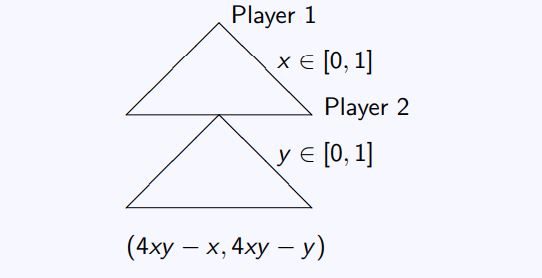
\includegraphics[width=0.55\linewidth]{images/DR5-Slide31}
\caption{}
\label{fig:DR5-Slide31}
\end{figure}

(4xy − x, 4xy − y)
%-----------------------------------------------------------%
%%  31 / 45
\subsection{The Concepts of Complete Information and Perfect
	Information}
\begin{itemize}
	\item A game is a game with complete information if both players
	know both the actions available to the other players and the
	payoffs obtained by other players under all the possible
	combinations of strategies.
\item 	In addition, if each player always knows which node of the
	extensive form of the game he/she is at when he/she has to make
	a move, then such a game is a game with perfect information.
\end{itemize}


%-----------------------------------------------------------%
%-----------------------------------------------------------%
%% 32 / 45
%%- \subsection{The Concepts of Complete Information and Perfect Information}
\begin{itemize}
	\item For example, chess is a game of perfect information (given a payoff
	structure of 1 point for a win, 0.5 for a draw, 0 for a loss), since
	the state of the game is always known, each player knows which
	moves are available to the opponent.
\item Bridge is definitely not a game of perfect information, as e.g. the
	bidder does not know how the cards are split between his
	opponents. 
	\item However, it may be argued that it is a game of
	complete information, since the scoring system is well defined and
	players know what others are allowed to play given their hand and
	the bidding (\textit{a full description of a strategy would however be very
	complex}).
\end{itemize}


%-----------------------------------------------------------%
%% 33 / 45
\subsection{Solution of Games with Perfect Information}
\begin{itemize}
\item In games of perfect information, moves are made in succession and
each of the previous moves are known to each player.
\item Such games can be solved by recursion based on the extensive
form of the game.
\item Consider the asymmetric hawk-dove game given above. The final
move is made by Player 2. Given the move made by Player 1 (H or
D), Player 2 simply maximises his expected reward.
\item This defines Player 2’s optimal action after H and his optimal
action after D.
\end{itemize}


%-----------------------------------------------------------%
%% 34 / 45
%% \subsection{Solution of Games with Perfect Information}
\begin{itemize}
	\item Working backwards, Player 1 assumes that Player 2 will use his
	best response to her action.
	\item This defines the action that Player 1 should take.
	It follows that there always exists a solution to a game with perfect
	information.
	\item  Unless at any node a player is indifferent between the
	actions he/she can take, this solution will be unique.
	\item 	Any vector of payoffs corresponding to the solution of such a game
	is called a value of the game.
\end{itemize}

%% 35 / 45
\newpage
\subsection{The Asymmetric Hawk-Dove Game}



\begin{figure}[h!]
\centering
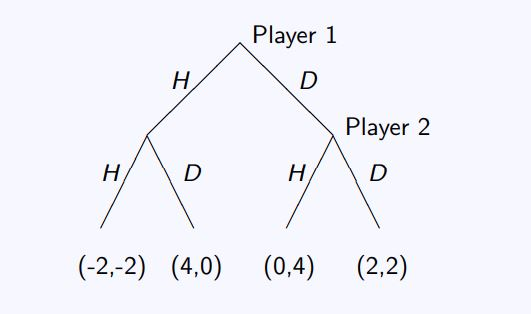
\includegraphics[width=0.6\linewidth]{images/DR5-Slide36}
\caption{}
\label{fig:DR5-Slide36}
\end{figure}

Player 2
(-2,-2) (4,0) (0,4) (2,2)

%-----------------------------------------------------------%
% 36 / 45
\subsection{Solution of Games with Perfect Information}
\begin{itemize}
	\item Suppose Player 1 has played H. Player 2 obtains -2 by playing H
	and 0 by playing D. Hence, his best response to H is to play D.
	Suppose Player 1 has played D. 
	\item Player 2 obtains 4 by playing H
	and 2 by playing D. Hence, his best response to D is H.
	Now we consider the action of Player 1.
\end{itemize}


%-----------------------------------------------------------%
% 37 / 45
%% \subsection{Solution of Games with Perfect Information}
\begin{itemize}
	\item If she plays H, then Player 2 will respond by playing D. Player 1
	obtains a reward of 4.
	\item 	If she plays D, then Player 2 will respond by playing H. Player 1
	obtains a reward of 0.
	\item 	It follows that Player 1 should play H. Player 2 follows by playing
	D.
	\item 	The value of the game is (4, 0).
	
\end{itemize}

%-----------------------------------------------------------%
%% 38 / 45
\subsection{Equilibrium Path and Subgame Perfect Equilibria}
\begin{itemize}
\item The set of actions observed at a solution of an extensive form
	game with perfect information is called an equilibrium path.
\item In the Hawk-Dove game considered above, the equilibrium path is
	(H, D).
\item However, such a path does not describe how players should react to
	”mistakes”, i.e. how should individuals act off the equilibrium path.
\item An equilibrium is said to be subgame perfect, if starting from any
	node on the game tree, players play an equilibrium pair of
	strategies, i.e. an equilibrium is played in any subgame of the game
	in question.
\end{itemize}


%-----------------------------------------------------------%
% 39 / 45
% \subsection{Equilibrium Path and Subgame Perfect Equilibria}
\begin{itemize}
\item In this case, the subgame perfect equilibrium is defined by giving
the optimal response of Player 2 to each action of Player 1 and the
optimal action of Player 1.
\item These were derived during the recursive solution of the game.
Player 2 should respond to H by playing D and respond to D by
playing H. Hence, Player 2’s subgame perfect equilibrium strategy
is (D|H, H|D).
\item The subgame perfect equilibrium strategy of Player 2 is H.
If nature has moves in a game of perfect information, then each
player is assumed to maximise his/her expected reward at each
stage of the recursion procedure.

\end{itemize}

%-----------------------------------------------------------%
%%% 40 / 45
\newpage
\section{Concepts of Pure and Mixed Strategies}
In games of perfect information, it is clear that unless a player is
indifferent between two actions, then he/she should never
randomise.
However, in games of imperfect information (e.g. when moves are
made simultaneously like rock-scissors-paper) it is clear that one
player may not want the other to ”guess” which action he/she is
going to take.
In such cases individuals choose the action they take at random,
i.e. they use a mixed strategy.

%-----------------------------------------------------------%
%%41 / 45
%% \subsection{Concepts of Pure and Mixed Strategies}
The matrix form of the rock-scissors-paper game is:
\begin{figure}[h!]
\centering
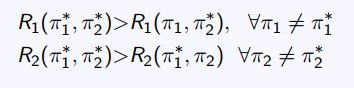
\includegraphics[width=0.7\linewidth]{images/DR7-Slide41}
\caption{}
\label{fig:DR7-Slide41}
\end{figure}

Intuitively, at equilibrium both players choose each action with a
probability of 1/3 (see tutorial sheet for details).

%-----------------------------------------------------------%
%%42 / 45
\subsection{Concepts of Pure and Mixed Strategies}
\begin{itemize}
	\item If a player always chooses the same action in a matrix game, then
	he/she is using a so called pure strategy.
	\item It is normally assumed that players choose their actions
	independently of each other (i.e. there is no communication).
	\item Later we will consider games in which players can communicate,
	i.e. the actions they take may be correlated.
\end{itemize}


%-----------------------------------------------------------%
%% 43 / 45
%% Concepts of Pure and Mixed Strategies
\begin{itemize}
	\item Suppose that in the rock-scissors-paper game, Player 1 plays rock,
	scissors and paper with probability pR, pS and pP, respectively.
\item Player 2 plays rock, scissors and paper with probability qR, qS and
	qP. The probability distribution over the set of strategy pairs is
\end{itemize}

\begin{figure}[h!]
\centering
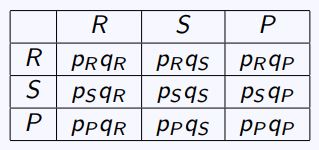
\includegraphics[width=0.5\linewidth]{images/DR5-Slide44}
\caption{}
\label{fig:DR5-Slide44}
\end{figure}

%-----------------------------------------------------------%
%% 44 / 45
%% Concepts of Pure and Mixed Strategies
When players use mixed strategies, the expected rewards of the
players can be calculated by taking expectations with respect to
the probability distribution over the set of strategy pairs. Hence,
\[R1(M1, M2)=pRqRR1(R, R) + pRqSR1(R, S) + pRqPR1(R, P) +
+pS qRR1(S, R) + pS qSR1(S, S) + pS qPR1(S, P) +
+pPqRR1(P, R) + pPqSR1(P, S) + pPqPR1(P, P)
=pRqS + pS qP + pPqR − pS qR − pPqS − pRqP.
\]
\newpage




\section{Solving Sequential Games Using Backwards Induction}
Below is a simple sequential game between two players. The labels with Player 1 and two within them are the information sets for players one or two, respectively. The numbers in the parentheses at the bottom of the tree are the payoffs at each respective point, in the format (Player 1, Player 2). The game is also sequential, so Player 1 makes the first decision (left or right) and Player 2 makes its decision after Player 1 (up or down).


\begin{figure}
	\centering
	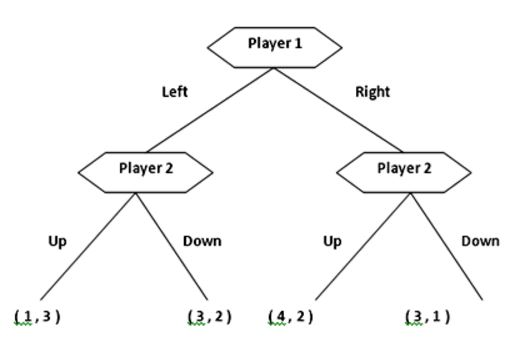
\includegraphics[width=0.7\linewidth]{images/BackwardInduction1}
	\caption{}
	\label{fig:BackwardInduction1}
\end{figure}
Backwards induction, like all game theory, uses the assumptions of rationality and maximization, meaning that Player 2 will maximize his payoff in any given situation. At either information set we have two choices, four in all. By eliminating the choices that Player 2 will not choose, we can narrow down our tree. In this way, we will bold the lines that maximize the player's payoff at the given information set.


\begin{figure}
	\centering
	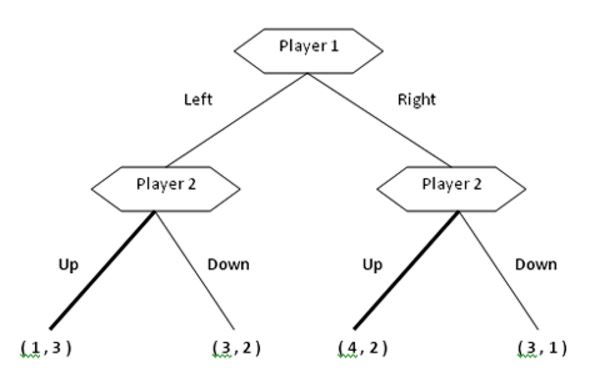
\includegraphics[width=0.7\linewidth]{images/BackwardInduction2}
	\caption{}
	\label{fig:BackwardInduction2}
\end{figure}
After this reduction, Player 1 can maximize its payoffs now that Player 2's choices are made known. The result is an equilibrium found by backwards induction of Player 1 choosing "right" and Player 2 choosing "up". Below is the solution to the game with the equilibrium path bolded.

\begin{figure}
	\centering
	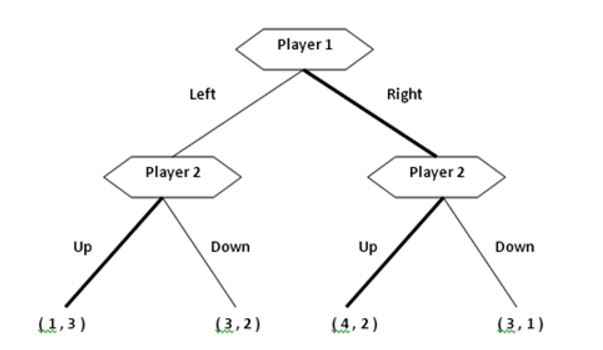
\includegraphics[width=0.7\linewidth]{images/BackwardInduction3}
	\caption{}
	\label{fig:BackwardInduction3}
\end{figure}
For example, one could easily set up a game similar to the one above using companies as the players. This game could include product release scenarios. If Company 1 wanted to release a product, what might Company 2 do in response? Will Company 2 release a similar competing product? By forecasting sales of this new product in different scenarios, we can set up a game to predict how events might unfold. Below is an alter-example of how one might model such a game.


\begin{figure}
\centering
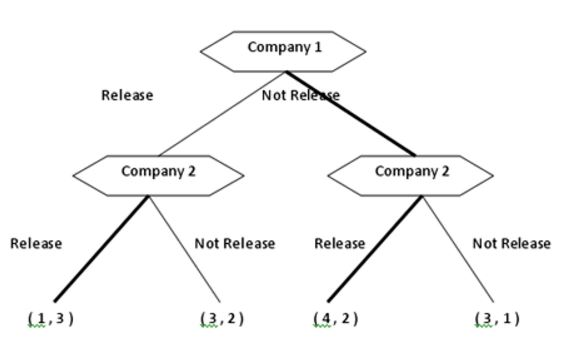
\includegraphics[width=0.7\linewidth]{images/BackwardInduction4}
\caption{}
\label{fig:BackwardInduction4}
\end{figure}

%----------------------------------------%
\subsection{Conclusion}
By using simple methods of game theory, we can solve for what would be a confusing array 
of outcomes in a real-world situation. Using game theory as a tool for financial analysis can be very helpful in sorting out potentially messy real-world situations, from mergers to product releases.


\chapter{Glossary}
\section{Glossary}

\begin{itemize}
	\item \textbf{Normal form game}
	A game in normal form is a function:
	
	${\displaystyle \pi \ :\prod _{i\in \mathrm {N} }\Sigma \ ^{i}\to \mathbb {R} ^{\mathrm {N} }} \pi \ :\prod _{i\in \mathrm {N} }\Sigma \ ^{i}\to \mathbb {R} ^{\mathrm {N} }$
	Given the tuple of strategies chosen by the players, one is given an allocation of payments (given as real numbers).
	
	A further generalization can be achieved by splitting the game into a composition of two functions:
	
	${\displaystyle \pi \ :\prod _{i\in \mathrm {N} }\Sigma \ ^{i}\to \Gamma \ } \pi \ :\prod _{i\in \mathrm {N} }\Sigma \ ^{i}\to \Gamma \ $
	the outcome function of the game (some authors call this function "the game form"), and:
	
	${\displaystyle \nu \ :\Gamma \ \to \mathbb {R} ^{\mathrm {N} }} \nu \ :\Gamma \ \to \mathbb {R} ^{\mathrm {N} }$
	the allocation of payoffs (or preferences) to players, for each outcome of the game.
	
	\item \textbf{Extensive form game}
	This is given by a tree, where at each vertex of the tree a different player has the choice of choosing an edge. The outcome set of an extensive form game is usually the set of tree leaves.
	
	\item \textbf{Cooperative game}
	A game in which players are allowed to form coalitions (and to enforce coalitionary discipline). A cooperative game is given by stating a value for every coalition:
	
	${\displaystyle \nu \ :2^{\mathbb {P} (N)}\to \mathbb {R} } \nu \ :2^{\mathbb {P} (N)}\to \mathbb {R} $
	It is always assumed that the empty coalition gains nil. Solution concepts for cooperative games usually assume that the players are forming the grand coalition ${\displaystyle N} N$, whose value ${\displaystyle \nu (N)} \nu (N) $ is then divided among the players to give an allocation.
	
	\item \textbf{Simple game}
	A Simple game is a simplified form of a cooperative game, where the possible gain is assumed to be either '0' or '1'. A simple game is couple (N, W), where W is the list of "winning" coalitions, capable of gaining the loot ('1'), and N is the set of players.
	
	\item Finite game 
	is a game with finitely many players, each of which has a finite set of strategies.
	Grand coalition 
	refers to the coalition containing all players. In cooperative games it is often assumed that the grand coalition forms and the purpose of the game is to find stable imputations.
	Mixed strategy 
	for player i is a probability distribution P on ${\displaystyle \Sigma \ ^{i}} \Sigma \ ^{i}$. It is understood that player i chooses a strategy randomly according to P.
	Mixed Nash Equilibrium 
	Same as Pure Nash Equilibrium, defined on the space of mixed strategies. Every finite game has Mixed Nash Equilibria.
	\item Pareto efficiency 
	An outcome a of game form π is (strongly) pareto efficient if it is undominated under all preference profiles.
	\item Preference profile 
	is a function ${\displaystyle \nu \ :\Gamma \ \to \mathbb {R} ^{\mathrm {N} }} \nu \ :\Gamma \ \to \mathbb {R} ^{\mathrm {N} }$. This is the ordinal approach at describing the outcome of the game. The preference describes how 'pleased' the players are with the possible outcomes of the game. See allocation of goods.
	\item Pure Nash Equilibrium 
	An element ${\displaystyle \sigma \ =(\sigma \ _{i})_{i\in \mathrm {N} }} \sigma \ =(\sigma \ _{i})_{i\in \mathrm {N} }$ of the strategy space of a game is a pure nash equilibrium point if no player i can benefit by deviating from his strategy ${\displaystyle \sigma \ _{i}} \sigma \ _{i}$, given that the other players are playing in ${\displaystyle \sigma \ } \sigma \$ . Formally:
	{\displaystyle \forall i\in \mathrm {N} \quad \forall \tau \ _{i}\in \ \Sigma \ ^{i}\quad \pi \ (\tau \ ,\sigma \ _{-i})\leq \pi \ (\sigma \ )} \forall i\in \mathrm {N} \quad \forall \tau \ _{i}\in \ \Sigma \ ^{i}\quad \pi \ (\tau \ ,\sigma \ _{-i})\leq \pi \ (\sigma \ )$.
	No equilibrium point is dominated.
	Say 
	%A player i has a Say if he is not a Dummy, i.e. if there is some tuple of complement strategies s.t. π (σ_i) is not a constant function.
	%Antonym: Dummy.
	
	\item Value 
	A value of a game is a rationally expected outcome. There are more than a few definitions of value, describing different methods of obtaining a solution to the game.
	\item Veto 
	A veto denotes the ability (or right) of some player to prevent a specific alternative from being the outcome of the game. A player who has that ability is called a veto player.
	Antonym: Dummy.
	
	\item Weakly acceptable game 
	is a game that has pure nash equilibria some of which are pareto efficient.
	\item Zero sum game 
	is a game in which the allocation is constant over different outcomes. Formally:
	${\displaystyle \forall \gamma \ \in \Gamma \ \sum _{i\in \mathrm {N} }\nu \ _{i}(\gamma \ )=const.} \forall \gamma \ \in \Gamma \ \sum _{i\in \mathrm {N} }\nu \ _{i}(\gamma \ )=const.$
	w.l.g. we can assume that constant to be zero. In a zero sum game, one player's gain is another player's loss. Most classical board games (e.g. chess, checkers) are zero sum.
	
\end{itemize}
\chapter{Mark Burke}
	\begin{center}
		\textbf{Game Theory %(  au Spaniel)
		}
	\end{center}

	
	\section{Analysis of (finite) Matrix Games}
	One of the best known games is \\
	
	{ \color{red} Prisoner's Dilemma (PD)} \vspace{3mm} \\
	
	\begin{center}
		{\color{blue}
			\begin{tabular}{c|c|c|c|}
				\multicolumn{2} {c} {} & \multicolumn{2}{c} {{\color{green}Player 2}} \\
				\cline{3-4}
				\multicolumn{2}{c|}{} & Keep Quiet         & Confess        \\
				\cline{2-4}
				\multirow{2} {*} {{\color{green}Player 1}}& Keep Quiet & (-1,-1) & (-12,0) \\
				\cline{2-4}
				& Confess &(0,-12)& (-8,-8) \\
				\cline{2-4}
				%C & (2,6) & (4,7)& (0,8) \\
				%\hline
			\end{tabular}
		}
	\end{center}
	
	The solution is $\langle$ confess, confess $\rangle$. (See IESDS). \\ Why don't the players coordinate to get $\langle$ Keep Quiet, Keep Quiet $\rangle$ ?
	
	The exact payoffs are irrelevant, the game can also be represented by the order of players' preferences  - most preferred (p1) to least preferred (p4) :
	\begin{center}
		{\color{blue}
			\begin{tabular}{c|c|c|c|}
				\multicolumn{2} {c} {} & \multicolumn{2}{c} {{\color{green}Player 2}} \\
				\cline{3-4}
				\multicolumn{2}{c|}{} & Keep Quiet         & Confess        \\
				\cline{2-4}
				\multirow{2} {*} {{\color{green}Player 1}}& Keep Quiet & (p2,p2) & (p4,p1) \\
				\cline{2-4}
				& Confess &(p1,p4)& (p3,p3) \\
				\cline{2-4}
				%C & (2,6) & (4,7)& (0,8) \\
				%\hline
			\end{tabular}
		}
	\end{center}
	
	Other examples of PD-like games are
	\begin{itemize}
		\item {\color{red} War} with strategies {\color{blue} Defend, Attack} respectively.
		\item {\color{red} Arms Race} with strategies {\color{blue} Pass, Build} respectively.
		\item {\color{red} Free Trade/ Protection} with strategies {\color{blue} No Tax, Tax} respectively.
		\item {\color{red} Advertising} with strategies {\color{blue} No Ads, Ads} respectively.
	\end{itemize}
	
	{ \color{red}Deadlock} is another game ( success is to fail!): \vspace{3mm} \\
	
	\begin{center}
		{\color{blue}
			\begin{tabular}{c|c|c|c|}
				\multicolumn{2} {c} {} & \multicolumn{2}{c} {{\color{green}Player 2}} \\
				\cline{3-4}
				\multicolumn{2}{c|}{} & Try         & Fail       \\
				\cline{2-4}
				\multirow{2} {*} {{\color{green}Player 1}}& Try & (0,0) & (-1,1) \\
				\cline{2-4}
				& Fail &(1,-1)& (0,0) \\
				\cline{2-4}
				%C & (2,6) & (4,7)& (0,8) \\
				%\hline
			\end{tabular}
		}
	\end{center}
	
	Using preferences, we can consider the more general version of deadlock
	\begin{center}
		{\color{blue}
			\begin{tabular}{c|c|c|c|}
				\multicolumn{2} {c} {} & \multicolumn{2}{c} {{\color{green}Player 2}} \\
				\cline{3-4}
				\multicolumn{2}{c|}{} & Left        & Right        \\
				\cline{2-4}
				\multirow{2} {*} {{\color{green}Player 1}}& Up & (p2,p2) & (p1,p4) \\
				\cline{2-4}
				& Down &(p4,p1)& (p3,p3) \\
				\cline{2-4}
				%C & (2,6) & (4,7)& (0,8) \\
				%\hline
			\end{tabular}
		}
	\end{center}
	The solution is $\langle$ Up, Left $\rangle$. (See IESDS). Neither player gets hir first choice unless the other makes a mistake.
	
\newpage	\subsection{Strict Dominance}
	
	\textit{Strategy X strictly dominates strategy Y for a player if X gives a bigger (more preferred) payoff than Y no matter what the other players do. Players never rationally choose strictly dominated strategies.}
	
	Reduce the matrix by \textbf{Iterated Elimination of Strictly Dominated Strategies} (IESDS) - see PD and Deadlock above. The order of elimination is irrelevant. Another example is the {\color{red} Dance Club} game:
	\begin{center}
		{\color{blue}
			\begin{tabular}{c|c|c|c|}
				\multicolumn{2} {c} {} & \multicolumn{2}{c} {{\color{green}Boon docks}} \\
				\cline{3-4}
				\multicolumn{2}{c|}{} &   Salsa       &  Hip Hop       \\
				\cline{2-4}
				\multirow{2} {*} {{\color{green}Downtown}}& Salsa & (80,0) & (60,40) \\
				\cline{2-4}
				& Hip Hop &(40,60)& (40,0) \\
				\cline{2-4}
				%C & (2,6) & (4,7)& (0,8) \\
				%\hline
			\end{tabular}
		}
	\end{center}
	The solution is $\langle$ Salsa, Hip Hop $\rangle$. Salsa dominates Hip Hop for Club Downtown, then Boonies choses Hip Hop.
	
	Some more examples
	
	\begin{center}
		{\color{blue}
			\begin{tabular}{c|c|c|c|c|}
				\multicolumn{2} {c} {} & \multicolumn{3}{c} {{\color{green}Player 2}} \\
				\cline{3-5}
				\multicolumn{2}{c|}{} & Left        & Centre & Right        \\
				\cline{2-5}
				\multirow{3} {*} {{\color{green}Player 1}}& Up & (13,3) & (1,4)  & (7, 3)\\
				\cline{2-5}
				& Middle &(4,1)& (3,3) & (6,2) \\
				\cline{2-5}
				& Down & (-1,9) & (2,8)& (8,-1) \\
				\cline{2-5}
			\end{tabular}
		}
	\end{center}
	Denoting strict dominance by $>$, then in the order given C $>$ R,  M $>$ D, C $>$ L, M $>$ U. Thus the solution is $\langle$ Middle, Centre $\rangle$.
	
	{\color{red} Cournot Duopoly game}. Firm 1 can produce $i$ units at a cost of \euro 1 each. Similarly firm 2 can produce $j$ units at a cost of \euro 1 each. The units sell on the market at a price of \euro $[8-2(i+j)]^{+}$ each, where $[ . ]^{+}$ is the positive part of $[.]$ The payoff to firm 1 is the profit gained  which is \euro $ [8-2(i+j)]^{+}i - i$. Similarly the payoff to firm 2 is \euro $[8-2 (i+j)]^{+}j-j$. The game matrix is
	\begin{center}
		{\color{blue}
			\begin{tabular}{c|c|c|c|c|c|}
				\multicolumn{2} {c} {} & \multicolumn{4}{c} {{\color{green}Firm 2}} \\
				\cline{3-6}
				\multicolumn{2}{c|}{} & $j = 0$        & $j = 1$ & $j = 2$  &  $j = 3$    \\
				\cline{2-6}
				\multirow{4} {*} {{\color{green}Firm 1}}& $i=0$ & (0,0) & (0,5)  & (0, 6)& (0,1)\\
				\cline{2-6}
				& $i=1$ &(5,0)& (3,3) & (1,2)& (-1,-3)\\
				\cline{2-6}
				& $i=2$ & (6,0) & (2,1)& (-2,-2)& (-2,-3) \\
				\cline{2-6}
				& $i=3$ & (1,0)& (-3,-1)& (-3,-2) & (-3,-3) \\
				\cline{2-6}
			\end{tabular}
		}
	\end{center}
	The solution is $\langle i=1, j=1\rangle$. What is the sequence of eliminations that leads to this?
	
	All routes lead to the same result (proof?):
	\begin{center}
		{\color{blue}
			\begin{tabular}{c|c|c|c|}
				\multicolumn{2} {c} {} & \multicolumn{2}{c} {{\color{green}Player 2}} \\
				\cline{3-4}
				\multicolumn{2}{c|}{} & Left        & Right        \\
				\cline{2-4}
				\multirow{3} {*} {{\color{green}Player 1}}& Up & (1,-1) & (4,2)  \\
				\cline{2-4}
				& Middle &(0,2)& (3,3)  \\
				\cline{2-4}
				& Down & (-2,-2) & (2,-1) \\
				\cline{2-4}
			\end{tabular}
		}
	\end{center}
	The solution is $\langle$ Up, Right $\rangle$.
	
	\subsection{Weak Dominance} \label{M-WDS}
	\textit{Strategy X weakly dominates strategy Y for a player if X gives at least as big a payoff as Y no matter what the other players do and there is one at least one X payoff than is strictly greater than the corresponding Y payoff.}
	
	\textbf{Iterated Elimination of Weakly Dominated Strategies} (IEWDS) is in general not a valid technique. Consider the game:
	\begin{center}
		{\color{blue}
			\begin{tabular}{c|c|c|c|}
				\multicolumn{2} {c} {} & \multicolumn{2}{c} {{\color{green}Player 2}} \\
				\cline{3-4}
				\multicolumn{2}{c|}{} & Left        & Right        \\
				\cline{2-4}
				\multirow{3} {*} {{\color{green}Player 1}}& Up & (0,1) & (-4,2)  \\
				\cline{2-4}
				& Middle &(0,3)& (3,3)  \\
				\cline{2-4}
				& Down & (-2,2) & (3,-1) \\
				\cline{2-4}
			\end{tabular}
		}
	\end{center}
	If we proceed as before and denoting weak dominance by $\geq$, we  might argue that
	M $\geq$ U, L $\geq$ R. The solution is then $\langle$ Middle, Left $\rangle$. Alternatively we might argue that M $\geq$ D, R $\geq$ L which leads to the solution $\langle$ Middle, Right $\rangle$.
	

\newpage

	
\newpage
	\section{Best Response \& Nash Equilibrium}
	
	{ \color{red} Stag Hunt(SH)} - it requires cooperation to catch a stag! \vspace{3mm} \\
	
	\begin{center}
		{\color{blue}
			\begin{tabular}{c|c|c|c|}
				\multicolumn{2} {c} {} & \multicolumn{2}{c} {{\color{green}Player 2}} \\
				\cline{3-4}
				\multicolumn{2}{c|}{} & Stag         & Hare       \\
				\cline{2-4}
				\multirow{2} {*} {{\color{green}Player 1}}& Stag & ($3^*,3^*$) & (0,2) \\
				\cline{2-4}
				& Hare &(2,0)& ($1^*,1^*$) \\
				\cline{2-4}
				%C & (2,6) & (4,7)& (0,8) \\
				%\hline
			\end{tabular}
		}
	\end{center}
	For this game there is no SDS nor WDS.\\
	
	A \textbf{Nash equilibrium} (NE) is a set of strategies, one for each player, from which there is no incentive for any one player to deviate if all the other players play these strategies, i.e. no player can gain by changing, also called a ``No regrets'' choice. The \emph{Best Response} of a player to another player's choice of strategy is the strategy that gives the largest or best payoff. We'll denote this by placing an $^*$ beside the payoff, e.g. in the stag game above , ``stag'' with associated payoff 3 is the best response of player 1 to player 2 playing ``stag''. Hence if both parts of a payoff pair have asterisks beside them, this must be a pure strategy \textit{Nash} equilibrium (PSNE) - a pair of strategies where both players are playing deterministic strategies as opposed to a mixed strategy \textit{Nash} equilibrium (MSNE), where players are randomly mixing between the strategies available to them.\\
	
	Thus in the stag game, the PSNE solutions are $\langle$ stag, stag $\rangle$ and $\langle$ hare, hare $\rangle$. Notice that without efficient coordination, either solution is possible.
	
	Consider the ``Good buddies prisoner's dilemma'' game:
	\begin{center}
		{\color{blue}
			\begin{tabular}{c|c|c|c|}
				\multicolumn{2} {c} {} & \multicolumn{2}{c} {{\color{green}Player 2}} \\
				\cline{3-4}
				\multicolumn{2}{c|}{} & Keep Quiet        & Confess      \\
				\cline{2-4}
				\multirow{2} {*} {{\color{green}Player 1}}& Keep Quiet & (p1,p1) & (p4,p2) \\
				\cline{2-4}
				& Confess &(p2,p4)& (p3,p3) \\
				\cline{2-4}
				%C & (2,6) & (4,7)& (0,8) \\
				%\hline
			\end{tabular}
		}
	\end{center}
	This is identical to the stag hunt game.\\
	
	An alternative definition of a NE is ``mutual best response''. Some further examples:\\
	{ \color{red} Traffic Lights(TL)}   \vspace{3mm} \\
	
	\begin{center}
		{\color{blue}
			\begin{tabular}{c|c|c|c|}
				\multicolumn{2} {c} {} & \multicolumn{2}{c} {{\color{green}Car 2}} \\
				\cline{3-4}
				\multicolumn{2}{c|}{} & Go         & Stop      \\
				\cline{2-4}
				\multirow{2} {*} {{\color{green}Car 1}}& Go & (-5,-5) & (1,0) \\
				\cline{2-4}
				& Stop &(0,1)& (-1,-1) \\
				\cline{2-4}
				%C & (2,6) & (4,7)& (0,8) \\
				%\hline
			\end{tabular}
		}
	\end{center}
	The PSNE solutions are $\langle$ go, stop $\rangle$ and $\langle$ stop, go $\rangle$.\\
	
	{\color{red} Generals, Armies \& Battles}. Each general commands 3 armies. No battle occurs if either general puts 0 armies in the field. Otherwise the general with more armies wins the day. With $i$ and$j$ standing for the number of armies of General 1 and General 2 respectively in the battlefield, one possible game matrix is
	
	\begin{center}
		{\color{blue}
			\begin{tabular}{c|c|c|c|c|c|}
				\multicolumn{2} {c} {} & \multicolumn{4}{c} {{\color{green}General 2}} \\
				\cline{3-6}
				\multicolumn{2}{c|}{} & $j= 0$        & $j = 1$ & $j = 2$  &  $j = 3$    \\
				\cline{2-6}
				\multirow{4} {*} {{\color{green}General 1}}& $i=0$ & (0,0) & (0,0)  & (0, 0)& (0,0)\\
				\cline{2-6}
				& $i=1$ &(0,0)& (0,0) & (-1,1)& (-1,1)\\
				\cline{2-6}
				& $i=2$ & (0,0) & (1,-1)& (0,0)& (-1,1) \\
				\cline{2-6}
				& $i=3$ & (0,0)& (1,-1)& (1,-1) & (0,0) \\
				\cline{2-6}
			\end{tabular}
		}
	\end{center}
	What are the PSNE(s) ?
	
	\subsection{Dominance \& NE} \label{D-NE}
	
	If IESDS results in a unique solution then it is a (unique) NE. [proof by  appeal to ``no regrets'']. IESDS does not remove any NE.\\
	
	IEWDS may lose NE. It is necessary to check using e.g. Best Responses. If you have a choice eliminate SDS before WDS. Examples:
	\begin{itemize}
		\item The example of Section \ref{M-WDS} has two NE, each obtained by a different sequence of IEWDS.
		\item Consider the game
		\begin{center}
			{\color{blue}
				\begin{tabular}{c|c|c|c|}
					\multicolumn{2} {c} {} & \multicolumn{2}{c} {{\color{green}Player 2}} \\
					\cline{3-4}
					\multicolumn{2}{c|}{} & Left        & Right      \\
					\cline{2-4}
					\multirow{2} {*} {{\color{green}Player 1}}& Up & (2,3) & (4,3) \\
					\cline{2-4}
					& Down &(3,3)& (1,1) \\
					\cline{2-4}
					%C & (2,6) & (4,7)& (0,8) \\
					%\hline
				\end{tabular}
			}
		\end{center}
		Using IEWDS, L $\geq$ R, then D $>$ U. Hence the solution is $\langle$ Down, Left $\rangle$. But using Best Responses, another NE is $\langle$ Up, Right $\rangle$.
		\item The game
		\begin{center}
			{\color{blue}
				\begin{tabular}{c|c|c|c|c|}
					\multicolumn{2} {c} {} & \multicolumn{3}{c} {{\color{green}Player 2}} \\
					\cline{3-5}
					\multicolumn{2}{c|}{} & Left        & Centre & Right        \\
					\cline{2-5}
					\multirow{3} {*} {{\color{green}Player 1}}& Up & (2,2) & (4,2)  & (4, 3)\\
					\cline{2-5}
					& Middle &(2,4)& (5,5) & (7,3) \\
					\cline{2-5}
					& Down & (3,4) & (3,7)& (6,6) \\
					\cline{2-5}
				\end{tabular}
			}
		\end{center}
		Using IEWDS C $\geq$ L, then M $>$ U, M $>$ D and C$>$ R. Hence the solution is \\ $\langle$ Middle, Centre $\rangle$. This is the only NE.
	\end{itemize}
	
	
\newpage

	\section{MB2-MSNE}
	
	{ \color{red} Matching Pennies(MP)} is an example of a game with no PSNE.  \vspace{3mm} \\
	
	\begin{center}
		{\color{blue}
			\begin{tabular}{c|c|c|c|}
				\multicolumn{2} {c} {} & \multicolumn{2}{c} {{\color{green}Player 2}} \\
				\cline{3-4}
				\multicolumn{2}{c|}{} & Heads         & Tails      \\
				\cline{2-4}
				\multirow{2} {*} {{\color{green}Player 1}}& Heads & (1,-1) & (-1,1) \\
				\cline{2-4}
				& Tails &(-1,1)& (1,-1) \\
				\cline{2-4}
				%C & (2,6) & (4,7)& (0,8) \\
				%\hline
			\end{tabular}
		}
	\end{center}
	Other names for this game are
	\begin{itemize}
		\item Goalkeeeper v. Penalty Taker
		\item Offense v. Defense (American Football)
		\item Fastball v. Curveball (Baseball)
		\item Attack A or B v. Defend A or B
	\end{itemize}
	\textit{Nash} proved that every finite \footnote{finite number of players, finite number of pure strategies} game has a NE. \\ This game has the MSNE
	$\langle$ 1/2 Heads + 1/2 Tails, 1/2 Heads + 1/2 Tails $\rangle$.\\
	
	More generally, MSNEs can be found using the \textit{Bishop-Cannings} theorem. Consider the following game:
	\begin{center}
		{\color{blue}
			\begin{tabular}{c|c|c|c|}
				\multicolumn{2} {c} {} & \multicolumn{2}{c} {{\color{green}Player 2}} \\
				\cline{3-4}
				\multicolumn{2}{c|}{} & Left         & Right     \\
				\cline{2-4}
				\multirow{2} {*} {{\color{green}Player 1}}& Up & (3,-3) & (-2,2) \\
				\cline{2-4}
				& Down &(-1,1)& (0,0) \\
				\cline{2-4}
				%C & (2,6) & (4,7)& (0,8) \\
				%\hline
			\end{tabular}
		}
	\end{center}
	Again note that there is no PSNE. We'll use the notation $R_1 \langle s_1, s_2 \rangle $ and $R_2 \langle s_1, s_2\rangle $ to stand for the payoffs to Player 1 and 2 respectively when Player 1 plays strategy $s_1$ and Player 2 strategy $s_2$.
	\\ In the mixed strategy game let $p$ be the probability that Player 1 plays Up, and similarly $q$ the probability that Player 2 plays Left. Then the payoff to player 2  by playing Left against Player 1's mixed strategy is
	$$ R_2 \langle p \textrm{Up} + (1-p)\textrm{Down}, \textrm{Left}\rangle  = -3p + 1(1-p) $$
	Again the payoff to player 2 by playing Right against Player 1's mixed strategy is
	$$ R_2 \langle p \textrm{Up} + (1-p)\textrm{Down}, \textrm{Right}\rangle = 2p + 0(1-p) $$
	If the two payoff values are different then Player 2 has a definite preference between the two and so would not want to randomise. If for instance Player 2 were to choose Left, then Player 1 would abandon his mixed strategy and choose Up instead. Similarly if Player 2 were to choose Right instead, Player 1 would change from randomising to playing Down. In either case, the mixed strategies go out the window and no NE exists. To get a MSNE requires that Player 2 be indifferent between the two payoffs i.e. requires that the two payoffs be the same and since the the payoff at any mixed strategy is a linear combination of the pure strategy payoffs, this must also have the same value. Equating the two payoffs gives
	\begin{eqnarray*}
		% \nonumber to remove numbering (before each equation)
		-3p +1(1-p) &=& 2p + 0(1-p) \\
		\Rightarrow p &=& 1/6
	\end{eqnarray*}
	and the value of the payoff is
	$$ v_2 = R_2 \left\langle \frac{1}{6} \textrm{Up} + \frac{5}{6}\textrm{Down}, \textrm{Left or Right}\right\rangle  = \frac{1}{3} $$
	Similarly the payoffs to Player 1 by playing Up (respectively Down) against Player 2's mixed strategy are
	$$ R_1 \langle \textrm{Up}, q \textrm{Left} + (1-q)\textrm{Right}\rangle = 3q + (-2)(1-q) $$
	$$ R_1 \langle \textrm{Down}, q \textrm{Left} + (1-q)\textrm{Right} \rangle = (-1)q + 0(1-q) $$
	respectively. To be indifferent between the two requires
	\begin{eqnarray*}
		% \nonumber to remove numbering (before each equation)
		3q + (-2)(1-q) &=& (-1)q + 0(1-q) \\
		\Rightarrow q &=& 1/3
	\end{eqnarray*}
	and the value of the payoff is
	$$ v_1 = R_1 \left\langle \textrm{Up or Down}, \frac{1}{3} \textrm{Left} + \frac{2}{3}\textrm{Right}\right\rangle = -\frac{1}{3} $$
	
	Exercise: Show that the stag hunt game has a MSNE at $\langle$ 1/2 stag + 1/2 hare, 1/2 stag + 1/2 hare $\rangle$.\\
	
	We can have partial MSNE where (at least) one player has a pure strategy and (at least) one player has a mixed strategy.\\
	
	Examples of games with MSNE:
	\begin{itemize}
		\item { \color{red} Chicken} (aka {\color{magenta} Snowdrift}) :  \vspace{3mm} \\
		
		\begin{center}
			{\color{blue}
				\begin{tabular}{c|c|c|c|}
					\multicolumn{2} {c} {} & \multicolumn{2}{c} {{\color{green}Player 2}} \\
					\cline{3-4}
					\multicolumn{2}{c|}{} & Continue {\color{magenta}  / Stay in car }       & Swerve   {\color{magenta}  / Shovel }   \\
					\cline{2-4}
					\multirow{2} {*} {{\color{green}Player 1}}& Continue {\color{magenta}  / Stay in car }& (-10,-10) & (2,-2) \\
					\cline{2-4}
					& Swerve {\color{magenta}  / Shovel } &(-2,2)& (0,0) \\
					\cline{2-4}
					%C & (2,6) & (4,7)& (0,8) \\
					%\hline
				\end{tabular}
			}
		\end{center}
		PSNEs occur at $\langle$ Continue, Swerve $\rangle$ and at $\langle$ Swerve, Continue $\rangle$. There is also a MSNE at $\langle$ 1/5 continue + 4/5 swerve, 1/5 continue + 4/5 swerve $\rangle$. Show that $v_1 = v_2 = -2/5$.
		
		\item { \color{red} Battle of the Sexes}:  \vspace{3mm} \\
		
		\begin{center}
			{\color{blue}
				\begin{tabular}{c|c|c|c|}
					\multicolumn{2} {c} {} & \multicolumn{2}{c} {{\color{green}Her}} \\
					\cline{3-4}
					\multicolumn{2}{c|}{} & Ballet         & Fight      \\
					\cline{2-4}
					\multirow{2} {*} {{\color{green}Him}}& Ballet & (1,2) & (-1,1) \\
					\cline{2-4}
					& Fight &(-1,1)& (2,1) \\
					\cline{2-4}
					%C & (2,6) & (4,7)& (0,8) \\
					%\hline
				\end{tabular}
			}
		\end{center}
		PSNEs occur at $\langle$ Ballet, Ballet $\rangle$ and at $\langle$ Fight, Fight $\rangle$. Show that there is a MSNE at $\langle$ 1/3 ballet + 2/3 fight, 2/3 ballet + 1/3 fight $\rangle$ with $v_1= 2/3 = v_2$. Compare and contast this with the payoffs of the PSNEs.
	\end{itemize}
\newpage
\section{MB1-MSNE}
	
	{ \color{red} Matching Pennies(MP)} is an example of a game with no PSNE.  \vspace{3mm} \\
	
	\begin{center}
		{\color{blue}
			\begin{tabular}{c|c|c|c|}
				\multicolumn{2} {c} {} & \multicolumn{2}{c} {{\color{green}Player 2}} \\
				\cline{3-4}
				\multicolumn{2}{c|}{} & Heads         & Tails      \\
				\cline{2-4}
				\multirow{2} {*} {{\color{green}Player 1}}& Heads & (1,-1) & (-1,1) \\
				\cline{2-4}
				& Tails &(-1,1)& (1,-1) \\
				\cline{2-4}
				%C & (2,6) & (4,7)& (0,8) \\
				%\hline
			\end{tabular}
		}
	\end{center}
	Other names for this game are
	\begin{itemize}
		\item Goalkeeeper v. Penalty Taker
		\item Offense v. Defense (American Football)
		\item Fastball v. Curveball (Baseball)
		\item Attack A or B v. Defend A or B
	\end{itemize}
	\textit{Nash} proved that every finite \footnote{finite number of players, finite number of pure strategies} game has a NE. \\ This game has the MSNE
	$\langle$ 1/2 Heads + 1/2 Tails, 1/2 Heads + 1/2 Tails $\rangle$.\\
	
	More generally, MSNEs can be found using the \textit{Bishop-Cannings} theorem. Consider the following game:
	\begin{center}
		{\color{blue}
			\begin{tabular}{c|c|c|c|}
				\multicolumn{2} {c} {} & \multicolumn{2}{c} {{\color{green}Player 2}} \\
				\cline{3-4}
				\multicolumn{2}{c|}{} & Left         & Right     \\
				\cline{2-4}
				\multirow{2} {*} {{\color{green}Player 1}}& Up & (3,-3) & (-2,2) \\
				\cline{2-4}
				& Down &(-1,1)& (0,0) \\
				\cline{2-4}
				%C & (2,6) & (4,7)& (0,8) \\
				%\hline
			\end{tabular}
		}
	\end{center}
	Again note that there is no PSNE. We'll use the notation $R_1 \langle s_1, s_2 \rangle $ and $R_2 \langle s_1, s_2\rangle $ to stand for the payoffs to Player 1 and 2 respectively when Player 1 plays strategy $s_1$ and Player 2 strategy $s_2$.
	\\ In the mixed strategy game let $p$ be the probability that Player 1 plays Up, and similarly $q$ the probability that Player 2 plays Left. Then the payoff to player 2  by playing Left against Player 1's mixed strategy is
	$$ R_2 \langle p \textrm{Up} + (1-p)\textrm{Down}, \textrm{Left}\rangle  = -3p + 1(1-p) $$
	Again the payoff to player 2 by playing Right against Player 1's mixed strategy is
	$$ R_2 \langle p \textrm{Up} + (1-p)\textrm{Down}, \textrm{Right}\rangle = 2p + 0(1-p) $$
	If the two payoff values are different then Player 2 has a definite preference between the two and so would not want to randomise. If for instance Player 2 were to choose Left, then Player 1 would abandon his mixed strategy and choose Up instead. Similarly if Player 2 were to choose Right instead, Player 1 would change from randomising to playing Down. In either case, the mixed strategies go out the window and no NE exists. To get a MSNE requires that Player 2 be indifferent between the two payoffs i.e. requires that the two payoffs be the same and since the the payoff at any mixed strategy is a linear combination of the pure strategy payoffs, this must also have the same value. Equating the two payoffs gives
	\begin{eqnarray*}
		% \nonumber to remove numbering (before each equation)
		-3p +1(1-p) &=& 2p + 0(1-p) \\
		\Rightarrow p &=& 1/6
	\end{eqnarray*}
	and the value of the payoff is
	$$ v_2 = R_2 \left\langle \frac{1}{6} \textrm{Up} + \frac{5}{6}\textrm{Down}, \textrm{Left or Right}\right\rangle  = \frac{1}{3} $$
	Similarly the payoffs to Player 1 by playing Up (respectively Down) against Player 2's mixed strategy are
	$$ R_1 \langle \textrm{Up}, q \textrm{Left} + (1-q)\textrm{Right}\rangle = 3q + (-2)(1-q) $$
	$$ R_1 \langle \textrm{Down}, q \textrm{Left} + (1-q)\textrm{Right} \rangle = (-1)q + 0(1-q) $$
	respectively. To be indifferent between the two requires
	\begin{eqnarray*}
		% \nonumber to remove numbering (before each equation)
		3q + (-2)(1-q) &=& (-1)q + 0(1-q) \\
		\Rightarrow q &=& 1/3
	\end{eqnarray*}
	and the value of the payoff is
	$$ v_1 = R_1 \left\langle \textrm{Up or Down}, \frac{1}{3} \textrm{Left} + \frac{2}{3}\textrm{Right}\right\rangle = -\frac{1}{3} $$
	
	Exercise: Show that the stag hunt game has a MSNE at $\langle$ 1/2 stag + 1/2 hare, 1/2 stag + 1/2 hare $\rangle$.\\
	
	We can have partial MSNE where (at least) one player has a pure strategy and (at least) one player has a mixed strategy.\\
	
	Examples of games with MSNE:
	\begin{itemize}
		\item { \color{red} Chicken} (aka {\color{magenta} Snowdrift}) :  \vspace{3mm} \\
		
		\begin{center}
			{\color{blue}
				\begin{tabular}{c|c|c|c|}
					\multicolumn{2} {c} {} & \multicolumn{2}{c} {{\color{green}Player 2}} \\
					\cline{3-4}
					\multicolumn{2}{c|}{} & Continue {\color{magenta}  / Stay in car }       & Swerve   {\color{magenta}  / Shovel }   \\
					\cline{2-4}
					\multirow{2} {*} {{\color{green}Player 1}}& Continue {\color{magenta}  / Stay in car }& (-10,-10) & (2,-2) \\
					\cline{2-4}
					& Swerve {\color{magenta}  / Shovel } &(-2,2)& (0,0) \\
					\cline{2-4}
					%C & (2,6) & (4,7)& (0,8) \\
					%\hline
				\end{tabular}
			}
		\end{center}
		PSNEs occur at $\langle$ Continue, Swerve $\rangle$ and at $\langle$ Swerve, Continue $\rangle$. There is also a MSNE at $\langle$ 1/5 continue + 4/5 swerve, 1/5 continue + 4/5 swerve $\rangle$. Show that $v_1 = v_2 = -2/5$.
		
		\item { \color{red} Battle of the Sexes}:  \vspace{3mm} \\
		
		\begin{center}
			{\color{blue}
				\begin{tabular}{c|c|c|c|}
					\multicolumn{2} {c} {} & \multicolumn{2}{c} {{\color{green}Her}} \\
					\cline{3-4}
					\multicolumn{2}{c|}{} & Ballet         & Fight      \\
					\cline{2-4}
					\multirow{2} {*} {{\color{green}Him}}& Ballet & (1,2) & (-1,1) \\
					\cline{2-4}
					& Fight &(-1,1)& (2,1) \\
					\cline{2-4}
					%C & (2,6) & (4,7)& (0,8) \\
					%\hline
				\end{tabular}
			}
		\end{center}
		PSNEs occur at $\langle$ Ballet, Ballet $\rangle$ and at $\langle$ Fight, Fight $\rangle$. Show that there is a MSNE at $\langle$ 1/3 ballet + 2/3 fight, 2/3 ballet + 1/3 fight $\rangle$ with $v_1= 2/3 = v_2$. Compare and contast this with the payoffs of the PSNEs.
	\end{itemize}

\newpage
	\subsection{MSNE and Dominance}
	
	A SDS cannot be played with positive probability in a MSNE (otherwise a higher payoff can be obtained by not playing the SDS when the strategy says to play it).
	
\newpage

	\subsection{Strict Dominance in Mixed Strategies}
	Consider the game:
	\begin{center}
		{\color{blue}
			\begin{tabular}{c|c|c|c|}
				\multicolumn{2} {c} {} & \multicolumn{2}{c} {{\color{green}Player 2}} \\
				\cline{3-4}
				\multicolumn{2}{c|}{} & Left        & Right        \\
				\cline{2-4}
				\multirow{3} {*} {{\color{green}Player 1}}& Up & (3,-1) & (-1,1)  \\
				\cline{2-4}
				& Middle &(0,0)& (0,0)  \\
				\cline{2-4}
				& Down & (-1,2) & (2,-1) \\
				\cline{2-4}
			\end{tabular}
		}
	\end{center}
	This game has no SDS dominated by a pure strategy nor any PSNE. If a mixture of two pure strategies dominates another, then that strategy is a SDS.\\ In the above game 1/2 Up + 1/2 Down $>$ Middle. Remove Middle to get
	\begin{center}
		{\color{blue}
			\begin{tabular}{c|c|c|c|}
				\multicolumn{2} {c} {} & \multicolumn{2}{c} {{\color{green}Player 2}} \\
				\cline{3-4}
				\multicolumn{2}{c|}{} & Left         & Right      \\
				\cline{2-4}
				\multirow{2} {*} {{\color{green}Player 1}}& Up & (3,-1) & (-1,1) \\
				\cline{2-4}
				& Down &(-1,2)& (2,-1) \\
				\cline{2-4}
				%C & (2,6) & (4,7)& (0,8) \\
				%\hline
			\end{tabular}
		}
	\end{center}
	Show that a MSNE exists at $\langle$ (3/5)Up + (2/5)Down, (3/7)Left + (4/7)Right $\rangle$.\\
	
	Another example:
	\begin{center}
		{\color{blue}
			\begin{tabular}{c|c|c|c|c|}
				\multicolumn{2} {c} {} & \multicolumn{3}{c} {{\color{green}Player 2}} \\
				\cline{3-5}
				\multicolumn{2}{c|}{} & Left        & Centre & Right        \\
				\cline{2-5}
				\multirow{3} {*} {{\color{green}Player 1}}& Up & (-3,6) & (9,1)  & (0, 2)\\
				\cline{2-5}
				& Middle &(3,-4)& (2,4) & (4,1) \\
				\cline{2-5}
				& Down & (4,7) & (3,2)& (-3,2) \\
				\cline{2-5}
			\end{tabular}
		}
	\end{center}
	Using IESDS, we get (1/4)L + (3/4)C $>$ R, D $>$ M, L $>$ C, D $>$ U. Thus the solution is $\langle$ Down, Left $\rangle$.
	
\newpage
	\subsection{Atypical Matrix Games}
	Almost all matrix games have an odd number of solutions (Wilson 1971). Examples of non generic games follow. Weak dominance is usually the culprit.
	\begin{itemize}
		\item \textit{}
		\begin{center}
			{\color{blue}
				\begin{tabular}{c|c|c|c|}
					\multicolumn{2} {c} {} & \multicolumn{2}{c} {{\color{green}Player 2}} \\
					\cline{3-4}
					\multicolumn{2}{c|}{} & Left         & Right      \\
					\cline{2-4}
					\multirow{2} {*} {{\color{green}Player 1}}& Up & (1,1) & (0,0) \\
					\cline{2-4}
					& Down &(0,0)& (0,0) \\
					\cline{2-4}
					%C & (2,6) & (4,7)& (0,8) \\
					%\hline
				\end{tabular}
			}
		\end{center}
		There are two PSNEs.
		\item\textit{}
		\begin{center}
			{\color{blue}
				\begin{tabular}{c|c|c|c|}
					\multicolumn{2} {c} {} & \multicolumn{2}{c} {{\color{green}Player 2}} \\
					\cline{3-4}
					\multicolumn{2}{c|}{} & Left         & Right      \\
					\cline{2-4}
					\multirow{2} {*} {{\color{green}Player 1}}& Up & (2,2) & (9,0) \\
					\cline{2-4}
					& Down &(2,3)& (5,-1) \\
					\cline{2-4}
					%C & (2,6) & (4,7)& (0,8) \\
					%\hline
				\end{tabular}
			}
		\end{center}
		Using IESDS, L $>$ R. Player 1 can choose Up or Down as pure strategies or any mixture of the two. All strategies yield a payoff of 2: an infinite number of strategies.\\
		If tempted to use IEWDS, U $\geq$ D, leading to the solution $\langle$ Up, Right $\rangle$. Caveat emptor!
		\item Example 2 of Section \ref{D-NE} had two PSNEs. It also has an infinite number of MSNEs at $\langle$ Up, $q$Left + $(1-q)$Right $\rangle$ for $ q \leq 3/4$.
		\item { \color{red} \textit{Selten}'s Horse}:  \vspace{3mm} \\
		
		\begin{center}
			{\color{blue}
				\begin{tabular}{c|c|c|c|}
					\multicolumn{2} {c} {} & \multicolumn{2}{c} {{\color{green}Player 2}} \\
					\cline{3-4}
					\multicolumn{2}{c|}{} & Left         & Right      \\
					\cline{2-4}
					\multirow{2} {*} {{\color{green}Player 1}}& Up & (3,1) & (0,0) \\
					\cline{2-4}
					& Down &(2,2)& (2,2) \\
					\cline{2-4}
					%C & (2,6) & (4,7)& (0,8) \\
					%\hline
				\end{tabular}
			}
		\end{center}
		There are two PSNEs at $\langle$ Up,Left $\rangle$ and $\langle$ Down,Right $\rangle$ and an infinite number of MSNEs at $\langle$ Down, $q$Left + $(1-q)$Right $\rangle$ for $ q \leq 2/3$.
		
		\item { \color{red} Take or Share} - TV game show:  \vspace{3mm} \\
		
		\begin{center}
			{\color{blue}
				\begin{tabular}{c|c|c|c|}
					\multicolumn{2} {c} {} & \multicolumn{2}{c} {{\color{green}Player 2}} \\
					\cline{3-4}
					\multicolumn{2}{c|}{} & Share         & Take     \\
					\cline{2-4}
					\multirow{2} {*} {{\color{green}Player 1}}& Share & (4,4) & (0,8) \\
					\cline{2-4}
					& Take &(8,0)& (0,0) \\
					\cline{2-4}
					%C & (2,6) & (4,7)& (0,8) \\
					%\hline
				\end{tabular}
			}
		\end{center}
		There are three PSNEs at all but $\langle$ Share, Share $\rangle$.
		If one player chooses Take, then the other is indifferent between Share and Take which leads to an infinity of MSNEs.
	\end{itemize}
	

	

	
	
	\newpage
	\subsection{Atypical Matrix Games}
	Almost all matrix games have an odd number of solutions (Wilson 1971). Examples of non generic games follow. Weak dominance is usually the culprit.
	\begin{itemize}
		\item \textit{}
		\begin{center}
			{\color{blue}
				\begin{tabular}{c|c|c|c|}
					\multicolumn{2} {c} {} & \multicolumn{2}{c} {{\color{green}Player 2}} \\
					\cline{3-4}
					\multicolumn{2}{c|}{} & Left         & Right      \\
					\cline{2-4}
					\multirow{2} {*} {{\color{green}Player 1}}& Up & (1,1) & (0,0) \\
					\cline{2-4}
					& Down &(0,0)& (0,0) \\
					\cline{2-4}
					%C & (2,6) & (4,7)& (0,8) \\
					%\hline
				\end{tabular}
			}
		\end{center}
		There are two PSNEs.
		\item\textit{}
		\begin{center}
			{\color{blue}
				\begin{tabular}{c|c|c|c|}
					\multicolumn{2} {c} {} & \multicolumn{2}{c} {{\color{green}Player 2}} \\
					\cline{3-4}
					\multicolumn{2}{c|}{} & Left         & Right      \\
					\cline{2-4}
					\multirow{2} {*} {{\color{green}Player 1}}& Up & (2,2) & (9,0) \\
					\cline{2-4}
					& Down &(2,3)& (5,-1) \\
					\cline{2-4}
					%C & (2,6) & (4,7)& (0,8) \\
					%\hline
				\end{tabular}
			}
		\end{center}
		Using IESDS, L $>$ R. Player 1 can choose Up or Down as pure strategies or any mixture of the two. All strategies yield a payoff of 2: an infinite number of strategies.\\
		If tempted to use IEWDS, U $\geq$ D, leading to the solution $\langle$ Up, Right $\rangle$. Caveat emptor!
		\item Example 2 of Section \ref{D-NE} had two PSNEs. It also has an infinite number of MSNEs at $\langle$ Up, $q$Left + $(1-q)$Right $\rangle$ for $ q \leq 3/4$.
		\item { \color{red} \textit{Selten}'s Horse}:  \vspace{3mm} \\
		
		\begin{center}
			{\color{blue}
				\begin{tabular}{c|c|c|c|}
					\multicolumn{2} {c} {} & \multicolumn{2}{c} {{\color{green}Player 2}} \\
					\cline{3-4}
					\multicolumn{2}{c|}{} & Left         & Right      \\
					\cline{2-4}
					\multirow{2} {*} {{\color{green}Player 1}}& Up & (3,1) & (0,0) \\
					\cline{2-4}
					& Down &(2,2)& (2,2) \\
					\cline{2-4}
					%C & (2,6) & (4,7)& (0,8) \\
					%\hline
				\end{tabular}
			}
		\end{center}
		There are two PSNEs at $\langle$ Up,Left $\rangle$ and $\langle$ Down,Right $\rangle$ and an infinite number of MSNEs at $\langle$ Down, $q$Left + $(1-q)$Right $\rangle$ for $ q \leq 2/3$.
		
		\item { \color{red} Take or Share} - TV game show:  \vspace{3mm} \\
		
		\begin{center}
			{\color{blue}
				\begin{tabular}{c|c|c|c|}
					\multicolumn{2} {c} {} & \multicolumn{2}{c} {{\color{green}Player 2}} \\
					\cline{3-4}
					\multicolumn{2}{c|}{} & Share         & Take     \\
					\cline{2-4}
					\multirow{2} {*} {{\color{green}Player 1}}& Share & (4,4) & (0,8) \\
					\cline{2-4}
					& Take &(8,0)& (0,0) \\
					\cline{2-4}
					%C & (2,6) & (4,7)& (0,8) \\
					%\hline
				\end{tabular}
			}
		\end{center}
		There are three PSNEs at all but $\langle$ Share, Share $\rangle$.
		If one player chooses Take, then the other is indifferent between Share and Take which leads to an infinity of MSNEs.
	\end{itemize}
	
	\section{Minimax Game Solution}
	An alternative to ``solving '' matrix games using the concept of \textit{Nash} Equilibrium is the Minimax approach. It was originally devised for 2-player ``Zero Sum'' or ``Constant Sum'' games whereby what one player gains the other player loses. Each player attempts to maximise hir payoff assuming that hir opponent is attempting to minimise it.\\
	
	Consider the constant sum game

	
\end{document}
